\documentclass[12pt,oneside,openany,a4paper]{book}

%中興大學LaTeX樣版設定區
%==========================================================================================================================
%版面設定
\usepackage{geometry}
\geometry{textheight=20.5cm,top=3cm,bottom=3cm,footskip=1.5cm, marginparwidth=2.5cm,left=3cm,right=3cm}

\usepackage{xeCJK}
\setCJKmainfont{TW-MOE-Std-Kai}

%章、節、小節名稱設定
\usepackage[small,sf,center]{titlesec}
\titleformat{\chapter}[hang]{\centering\Large\rm}{}{0.2cm}{}
\titlespacing{\chapter}{0cm}{5mm}{5mm}
\titleformat{\section}[hang]{\large\rm}{}{0.2cm}{}
\titlespacing{\section}{0cm}{3mm}{5mm}
\titleformat{\subsection}[hang]{\normalsize\rm}{}{0.3cm}{}
\titlespacing{\subsection}{0.5cm}{0.2cm}{0.2cm}
\renewcommand{\chaptername}{}
\renewcommand{\thechapter}{}
\renewcommand{\thesection}{}
\renewcommand{\thesubsection}{}


%設定各目次的標題
\usepackage{titletoc}
\renewcommand{\contentsname}{目錄}
\renewcommand{\listfigurename}{圖目次}
\renewcommand{\listtablename}{表目次}

%---------------------------------------------------
%設定圖表標題和排序方式
\usepackage{caption}
\renewcommand{\figurename}{圖}
\renewcommand{\tablename}{表}
% setting table and figure number list style,if your thesis need the style. ex:Table 3.5 or Fig 2.1
\renewcommand{\thetable}{\arabic{chapter}.\arabic{table}}
\renewcommand{\thefigure}{\arabic{chapter}.\arabic{figure}}
% the following is the other number list for table and figure.
%\renewcommand{\thetable}{\arabic{table}}
%\renewcommand{\thefigure}{\arabic{figure}}

%設定附錄標題
\usepackage{appendix}
\renewcommand{\appendixpagename}{\Large 附錄}

%設定超連的地字體
\usepackage{url}
\def\UrlFont{\rm}

%PDF的超連結套件
%列印時,請將colorlinks 設成 false,否則有超連結部份顏色會比較淺。
% \usepackage[pdftex,colorlinks=true,urlcolor=blue,bookmarks=false]{hyperref}
\usepackage[driverfallback=dvipdfm,colorlinks=true,urlcolor=blue,bookmarks=false]{hyperref}

%使用圖形的套件(jpg檔)
\usepackage{graphicx}
\graphicspath{{./figures/}}

%特殊符號與數學套件
\usepackage{pifont}
\usepackage{amsthm}
\usepackage{amsmath,amssymb}
%==========================================================================================================================

%其他樣版設定區
%==========================================================================================================================
%如需其他設定,請放在此區。
%==========================================================================================================================

\begin{document}

%內文基本設定
\pagestyle{plain}
\parindent=0.8cm
% \input mymacro
% \ctxfk
%==========================================================================================================================

%封面
\newpage
\thispagestyle{empty}
\begin{center}
    {\LARGE
        國立中興大學資訊管理學系\\
        碩士學位論文
    }
    \vspace{4.8cm}

    {\huge
        (中   文   論   文   題   目)
    }
    \vspace{2cm}

    {\LARGE
        (英   文   論   文   題   目)
    }
    \vspace{6.2cm}

    {\LARGE
        \begin{tabular}{lr}
          指導教授: & XXX \\
          研\hspace{0.33cm}究\hspace{0.33cm}生:& Y \space \space Y
        \end{tabular}
    }
    \vspace{2.9cm}

    {\LARGE
        中華民國115年01月
    }
\end{center}

%空白頁(題贈用)
\newpage
\thispagestyle{empty}
\begin{center}
\end{center}

%書名頁(中文)
\newpage
\thispagestyle{empty}
\begin{center}
    {\LARGE
        國立中興大學資訊管理學系\\
        碩士學位論文
    }
    \vspace{4.8cm}

    {\huge
        (中   文   論   文   題   目)
    }
    \vspace{2cm}

    {\LARGE
        (英   文   論   文   題   目)
    }
    \vspace{6.2cm}

    {\LARGE
        \begin{tabular}{lr}
          指導教授: & XXX \\
          研\hspace{0.33cm}究\hspace{0.33cm}生:& Y \space \space Y
        \end{tabular}
    }
    \vspace{2.9cm}

    {\LARGE
        中華民國115年01月
    }
\end{center}

\newpage
\thispagestyle{empty}
%==========================================================================================================================
\noindent 書名頁(英文)\\
英文書名頁內容(非必備,由各系所自行決定。)
%==========================================================================================================================

\newpage
\thispagestyle{empty}
\begin{center}
    {\LARGE{誌謝辭}}
\end{center}
%==========================================================================================================================
\begin{itemize}
    \item 在致謝辭之前需自行插入「審核頁」、「授權頁」(國家圖書館)和「授權頁」(本校圖書館)。
    \item 表達對師長、受訪者、同學、家人等感謝之意,以一頁為原則,最多不超過兩頁。\\
        (非必備,由各系所自行決定)
\end{itemize}
%==========================================================================================================================

\frontmatter
\begin{center}
    {\LARGE{中文摘要}}
\end{center}
%==========================================================================================================================
以一頁為原則,最多不超過兩頁,簡要說明研究動機、研究方法與設計、資料收集與分析、研究結果及討論建議等。
%==========================================================================================================================

\newpage
\begin{center}
    {\LARGE SUMMARY}
\end{center}
%==========================================================================================================================
精簡原則與中文摘要相同,必須注意專有名詞的翻譯是否正確。
%==========================================================================================================================

\newpage
\tableofcontents

\newpage
\listoftables
\listoffigures

\mainmatter

\chapter{壹、學位論文編印項目及次序}
    \begin{enumerate}
        \item[(一)] 封面
        \item[(二)] 空白頁
        \item[(三)] 書名頁(中文)
        \item[(四)] 書名頁(英文)*
        \item[(五)] 審核頁
        \item[(六)] 授權頁(國家圖書館)\\
                    授權頁(本校圖書館)
        \item[(七)] 誌謝辭*
        \item[(八)] 摘要(中文)
        \item[(九)] 摘要(英文)
        \item[(十)] 目次
        \item[(十一)] 圖表目次
        \item[(十二)] 正文
        \item[(十三)]  參考書目
        \begin{enumerate}
            \item[1.] 中文部分
            \begin{enumerate}
                \item[(1)] 圖書
                \item[(2)] 期刊論文
                \item[(3)] 網路資源
                \item[(4)] 其他
            \end{enumerate}
            \item[2.] 西文部分
            \begin{enumerate}
                \item[(1)] Books
                \item[(2)] Journal Articles
                \item[(3)] Electronic Resources
                \item[(4)] Others
            \end{enumerate}
        \end{enumerate}
    \end{enumerate}

\chapter{貳、學位論文各部分詳細規定}
\section{一、篇首部分}
\subsection{(一) 封面}
論文封面一律採橫式A4紙張大小,顏色則由各系所自行決定,平裝本字體顏色為黑色;
精裝本採燙金字。封面上下左右邊界各留3公分,內容應包括下列各項:
\begin{enumerate}
    \item 系所全名(以本校組織規程所列為準):國立中興大學XXXX學系或國立中興大學XXXX學研究所(標楷體20點字型,置中)
    \item 論文類別:碩士/博士學位論文 (標楷體20點字型,置中)
    \item 論文題目:一行無法容納時,應以倒三角形方式排列 (標楷體20點字型,置中),
           中文題目下方列英文題目(Times New Roman20點字型)
    \item 指導教授:xxx  xxx(與護照相同英文名)(標楷體20點字型,置中)
    \item 研究生:xxx xxx(與護照相同英文名)(標楷體20點字型,置中)
    \item 論文完成日期:中華民國xx年xx月,採中式數字 (標楷體20點字型,置中)(封面樣式見附錄一)。
\end{enumerate}

\subsection{(二) 空白頁}
封面後加入一張白色普通用紙,內容空白,做為題贈用。

\subsection{(三) 書名頁(中文)}
除了紙張為白色普通用紙之外,所有內容、形式與封面相同。視其需要可加一頁英文版。

\subsection{(四) 書名頁(英文)}
非必備,由各系所自行決定。

\subsection{(五) 審核頁}
此頁由各系(所)提供,經口試委員、指導教授簽名,以證明論文口試合格。(審核頁樣式見附錄二)

\subsection{(六) 授權頁}
是否授權本校、國家圖書館使用紙本論文之授權書置此。
另繳交本校之論文全文電子檔是否同意公開進行檢索、瀏覽、下載、列印之授權書得依研究生意願決定是否置此。(授權書樣式見附錄三)

\subsection{(七) 誌謝辭(非必備,由各系所自行決定)}
表達對師長、受訪者、同學、家人等感謝之意,以一頁為原則,最多不超過兩頁。

\subsection{(八) 中文摘要}
以一頁為原則,最多不超過兩頁,簡要說明研究動機、研究方法與設計、資料收集與分析、研究結果及討論建議等。

\subsection{(九) 英文摘要}
精簡原則與中文摘要相同,必須注意專有名詞的翻譯是否正確。

\subsection{(十) 目次}
按前述「論文編印項目次序」所列各項順序,依次註明章節編號、內容項目名稱及所在頁次,右邊對齊。

\subsection{(十一) 圖表目次}
註明圖表的編號、名稱及所在頁次,右邊對齊。表在前,圖在後。如圖或表總數超過10個以上,則分列表目次及圖目次。

\section{二、正文部分}
\subsection{(一) 論文編排}
\begin{enumerate}
    \item 論文以章為主體,每章均另起新頁,章標題(章名)置於版面頂端中央處。章下分節,不另起新頁,惟仍須居中排列。
    \item 章節編次使用一、二、三、$\cdots$等中文數字編號,章節與標題間空一格 (全型)。
    \item 各章節段落層次依序採用下列數序及縮格:\\
        \begin{tabular}{l}
        一、 \\
        $\triangle\triangle$ (一) 縮格二格 \\
        $\triangle\triangle\triangle\triangle$1. 縮格四格 \\
        $\triangle\triangle\triangle\triangle\triangle$(1) 縮格六格 \\
        $\triangle\triangle\triangle\triangle\triangle\triangle\triangle\triangle$\ding{172} 縮格八格 \\
        \end{tabular}
    \item 行距:中文間隔一行,每頁最少32行,英文間隔1.5行,每頁最少28行,章節名稱下留雙倍行距。
    \item 字距:中文為密集字距,每行最少32字。英文不拘。
\end{enumerate}

\subsection{(二) 圖表處理}
\begin{enumerate}
    \item 表、圖均須分別編列阿拉伯數字序號與標題,並各自成體系。其序數依照正文中之後次序為準。
    \item 表之序數與標題置於表之上方,並居中排列。
    \item 圖之序數與標題則置於圖之下方,同樣居中排列。
    \item 資料來源及說明一律置於表圖之下方,並齊左排列。
    \item 文內敘述涉及任何表、圖,應確切指明表或圖的序數,如「見表1」或「見圖1」,不宜使用「見下表」或「見下圖」。
    \item 表、圖在文內之安插宜選擇適當位置,通常置於首次陳述的段落之後,如遇實際需要,亦可另起一頁。惟均以置於版面中央為宜。
    \item 如圖表過大,可列印於大型紙張上,並以摺疊方式處理。
\end{enumerate}

\subsection{(三) 註釋}
\begin{enumerate}
    \item 註釋之格式不拘,依各學門習用者為準;置於各該附註出現之頁底、章節末(稱為Pagenote、Chapternote);或置於結論之後、參考書目之前(稱為Endnote)。
    \item 註釋置於正文之後,不需另起一頁。
    \item 引用或參考他人著作,均應使用註釋加以說明。
    \item 各章內連續編碼,各章之間不相接續。
\end{enumerate}

\section{三、參證部分}
\subsection{(一) 參考書目}
\begin{enumerate}
    \item 在正文撰述過程所徵引的所有參考文獻資料均應編製成參考書目置於本文之後,另起一頁,頁次接續正文編碼。內容首分中、西文,中文在前,西文在後;次分圖書、期刊論文、網路資源及其他。
    \item 參考書目之格式依各學門習用者為準,或採用MLA、Chicago Manual、American Psychological Association$\cdots\cdots$等格式。
\end{enumerate}

\subsection{(二) 附錄}
     凡屬大量數據或冗長資料,不便刊載於正文者,如原始資料(Raw data)、訪問記錄或問卷等,均可編為附錄置於參考書目之後,另起一頁,頁次接續參考書目編碼。

\section{四、其他}
\subsection{(一) 版面}
\begin{enumerate}
    \item 邊界︰設定上、下、左右邊界為3公分。
    \item 字型︰中英文字型由各院所自行規定。
\end{enumerate}

\subsection{(二) 頁碼}
\begin{enumerate}
    \item 頁碼位置應置於每頁的頁尾,對齊方式為置中。
    \item 摘要至正文前,以i、ii、iii$\cdots$等小寫羅馬數字連續編碼。
    \item 自正文第一章至附錄,均以1、2、3$\cdots$等阿拉伯數字連續編碼。
\end{enumerate}

\subsection{(三) 裝訂}
\begin{enumerate}
    \item 裝訂線在左方,書脊列印(1)本校及系所名稱(2)學位論文類別(3)論文名稱(4)著者姓名(5)畢業民國年月,採中式數字。
    \item 上述前四項資料列印時距上緣的距離各為3公分、9公分、12公分、19公分。至於畢業民國年月則由下往上留5公分。(書脊樣式見附錄四)
\end{enumerate}

\chapter{參、送繳紙本及上傳電子檔}
\section{一、送繳紙本}
通過論文口試之研究生應備妥經指導教授及論文考試委員簽名並加蓋系、所、
學位學程戳章之論文正本二冊繳交總圖書館,
其中一冊留存學校典藏,
另一冊分送有關單位典藏。

\section{二、上傳電子檔}
在辦理離校手續前,須登錄「中興大學電子學位論文服務系統」內,輸入論文基本資料,
上傳與紙本論文內容相同之論文全文電子檔供學校典藏與利用。

\chapter{肆、本樣版的使用方式}
\begin{enumerate}
    \item 至\href{http://www.miktex.org/}{ MiKTeX網站}下載 MiK\TeX ,並安裝「 Total」的MiK\TeX 套件。
    \item \href{http://www.amath.nchu.edu.tw/~u4815977/cwtex3.rar}{下載cw\TeX}。
    \item 將cwtex3.rar解壓縮後,點「cwtex-basic.exe」安裝\it{cw}\TeX (注意安裝時的訊息)。
    \item 將本樣版所在的資料夾複製到「d:$\backslash$tex」內。
    \item 將樣版(中文論文樣版檔名為NCHU\_Chinese.ctx、英文樣版檔名為NCHU\_English.ctx)另存新檔。
    \item 直接修改另存後之樣版內的標題與內容(封面請於ThesisTitle.ctx中修改)。
    \item 編譯流程:\it{cw}\TeX $\rightarrow$\LaTeX $\rightarrow$ \LaTeX $\rightarrow$ divpdfmx\\
        (因為需要產生目錄、相關的參考頁面或完成的PDF檔有超連結功能,所以需要點「\LaTeX 」兩次。)
    \item 在引入 .png or .jpg 圖檔時,必須先將圖檔 copy 到 c:$\backslash$xtemp 目錄中,然後產生 .bb檔,產生 .bb檔的方法請參考\it{cw}\TeX 排版系統 p.209頁。
    \item Mik\TeX 及\it{cw}\TeX 安裝過程,請參考應數系李政軒助教製作的\href{http://www.amath.nchu.edu.tw/~u4815977/How_to_Install_cwTeX/How_to_Install_cwTeX.html}{安裝教學網站}
\end{enumerate}

\chapter{伍、圖表範例}
\section{一、圖片範例}
\begin{figure}[h]
    \begin{center}
        
\includegraphics[bb=0 0 527 56,width=0.8\textwidth]{NCHU_Logo.jpg}
    \end{center}
    \caption{圖片範例}
\end{figure}

\section{二、表格範例}
\begin{table}[h]
    \caption{表格範例}
    \begin{center}
        \begin{tabular}{|c|c|}
        \hline
        % after \\: \hline or \cline{col1-col2} \cline{col3-col4} ...
        第一列第一行 & 第一列第二行 \\
        第二列第一行 & 第二列第二行 \\
        \hline
        \end{tabular}
    \end{center}
\end{table}

\backmatter
\chapter{參考文獻}
\renewcommand{\labelenumi}{[\arabic{enumi}]}
\begin{enumerate}
    \item 吳聰敏.吳聰慧(2005), 《cwTEX排版系統》,台北。
    \item Bringhurst, Robert (1996), {\it The Elements of Typographic Style}, Vancouver: Hartley \& Marks, 2nd edition.
\end{enumerate}

\appendix
\chapter{附錄一 : 封面樣式(一)}
    \begin{center}
        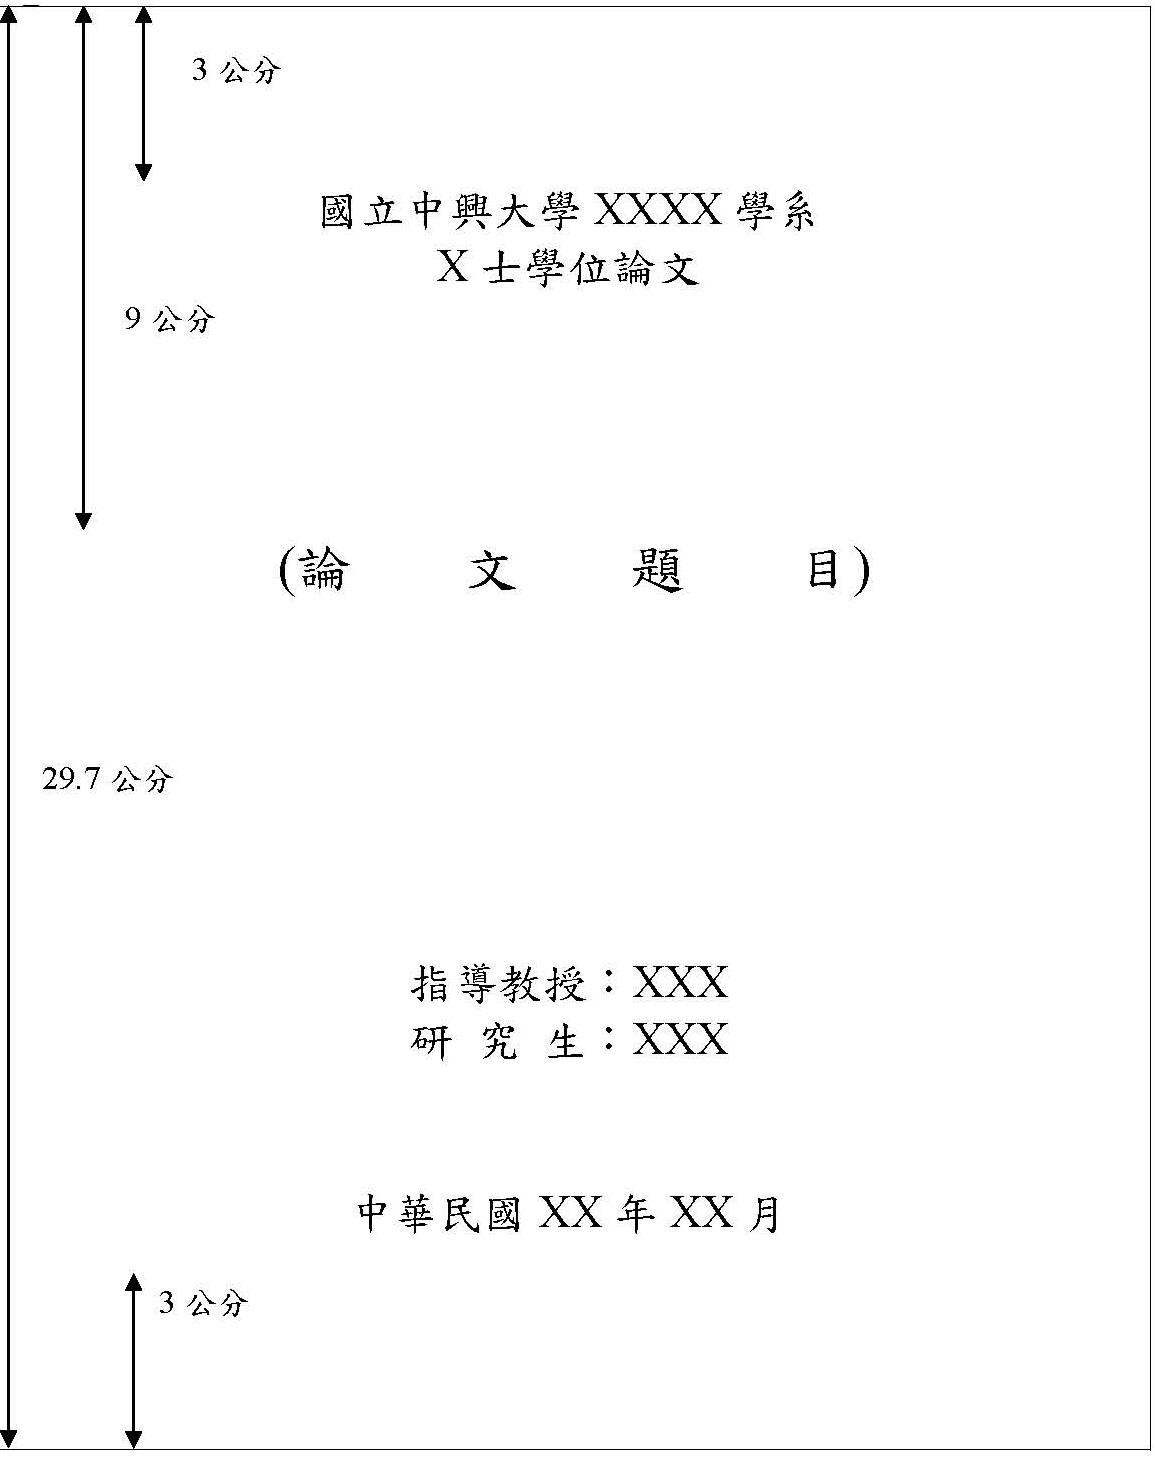
\includegraphics[bb=0 0 1155 1460,width=\textwidth]{TitlePage1.jpg}
    \end{center}

\chapter{附錄一 : 封面樣式(二)}
    \begin{center}
        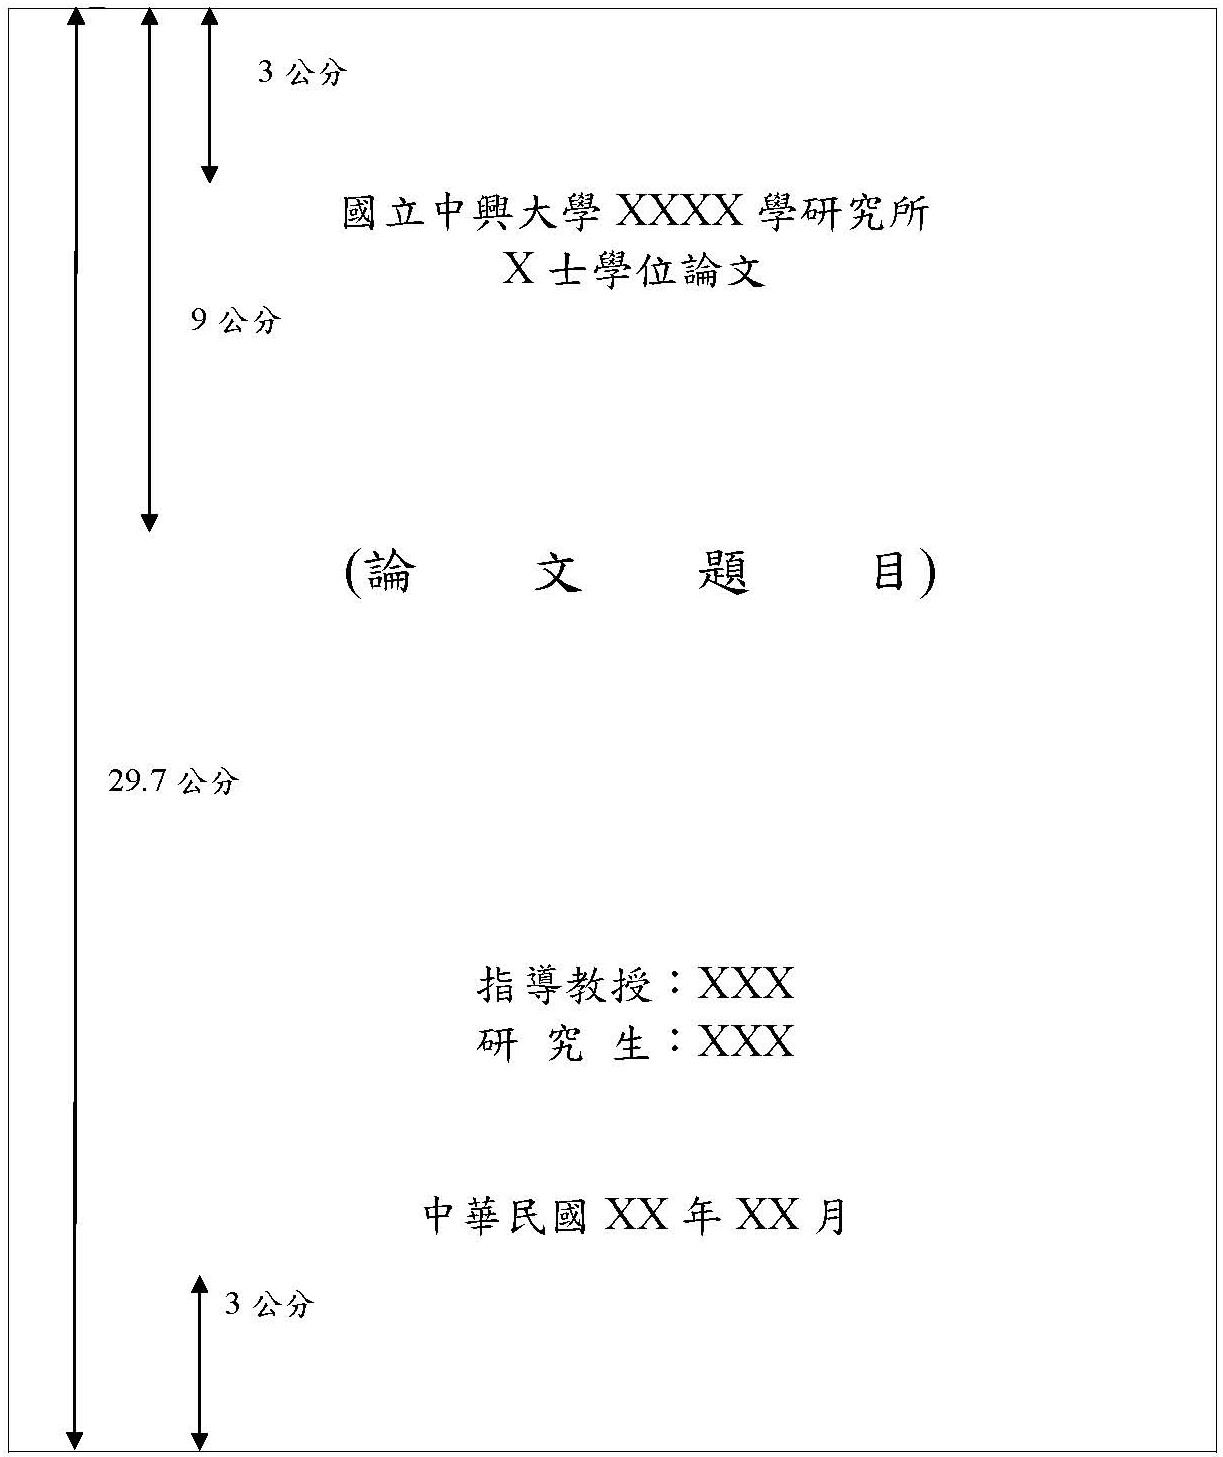
\includegraphics[bb=0 0 1223 1457,width=\textwidth]{TitlePage2.jpg}
    \end{center}

\chapter{附錄二 : 審核頁樣式(一)}
    \begin{center}
        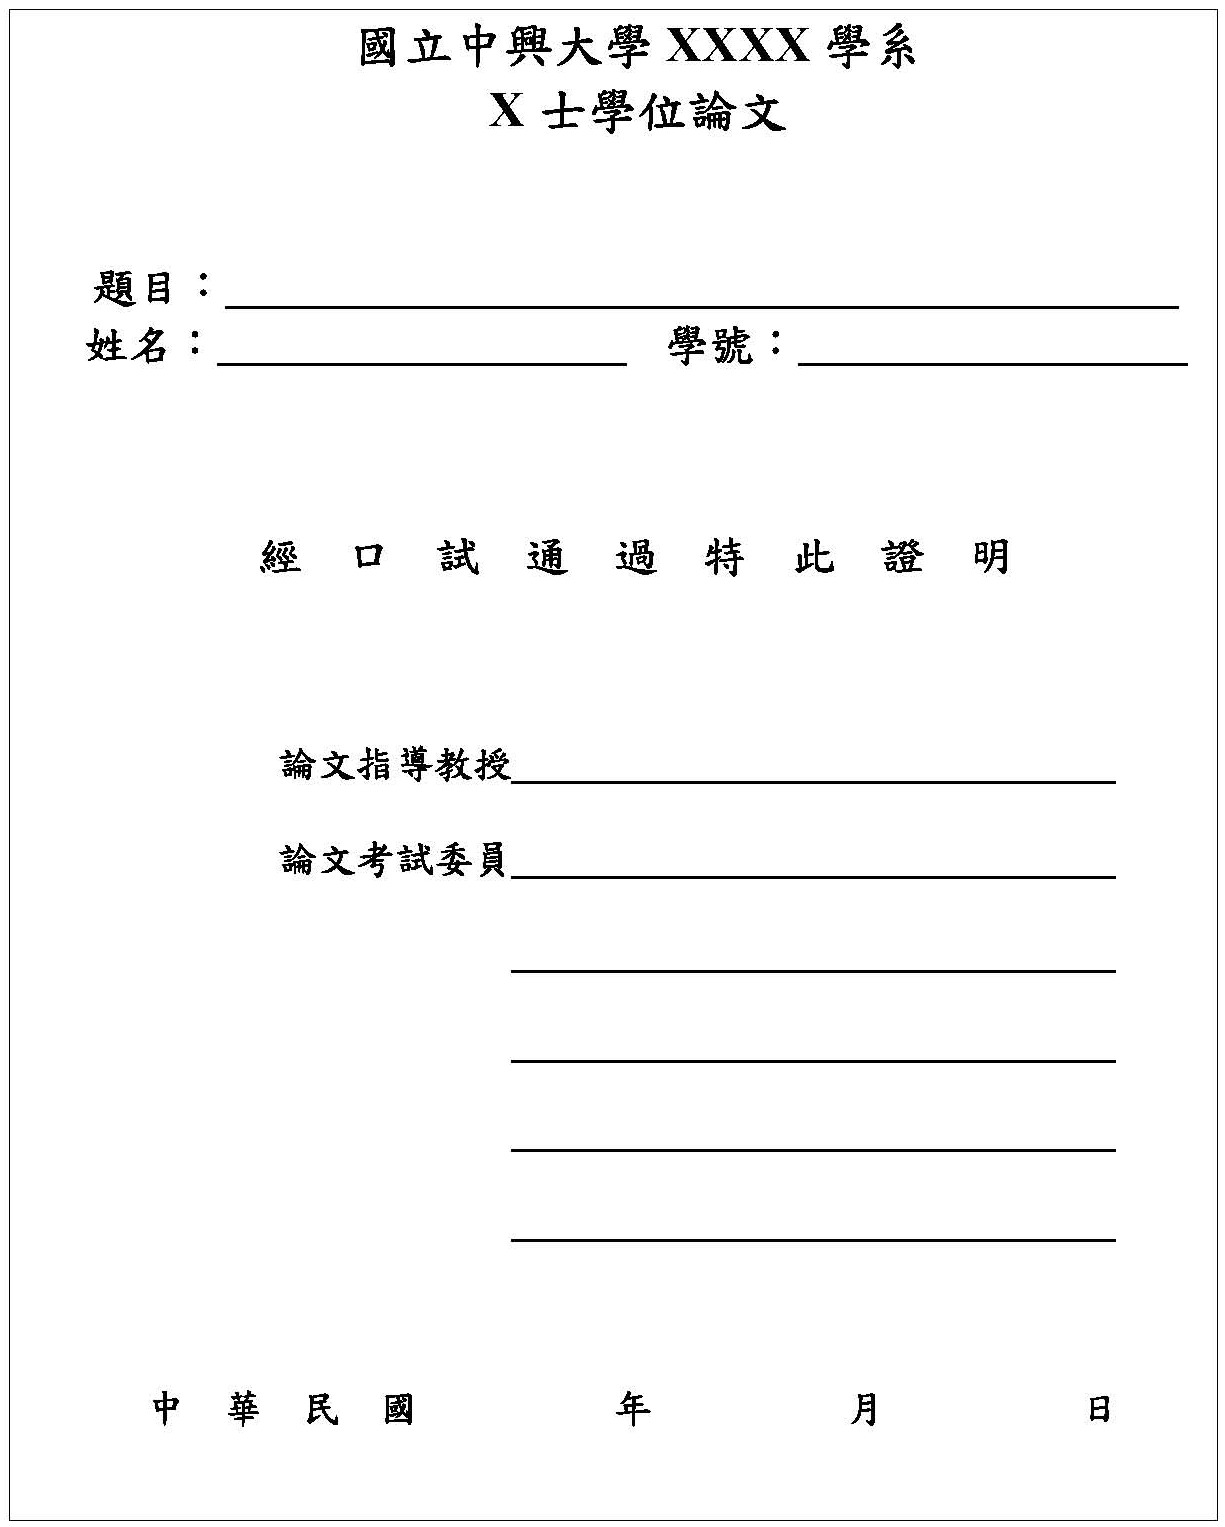
\includegraphics[bb=0 0 1225 1527,width=\textwidth]{examine1.jpg}
    \end{center}

\chapter{附錄二 : 審核頁樣式(二)}
    \begin{center}
        
\includegraphics[bb=0 0 1224 1527,width=\textwidth]{examine2.jpg}
    \end{center}

\chapter{附錄三 : 授權書樣式}
    \begin{center}
        
\includegraphics[bb=0 0 1341 1548,width=\textwidth]{authority.jpg}
    \end{center}

\chapter{附錄四 : 書脊樣式}
    \begin{center}
        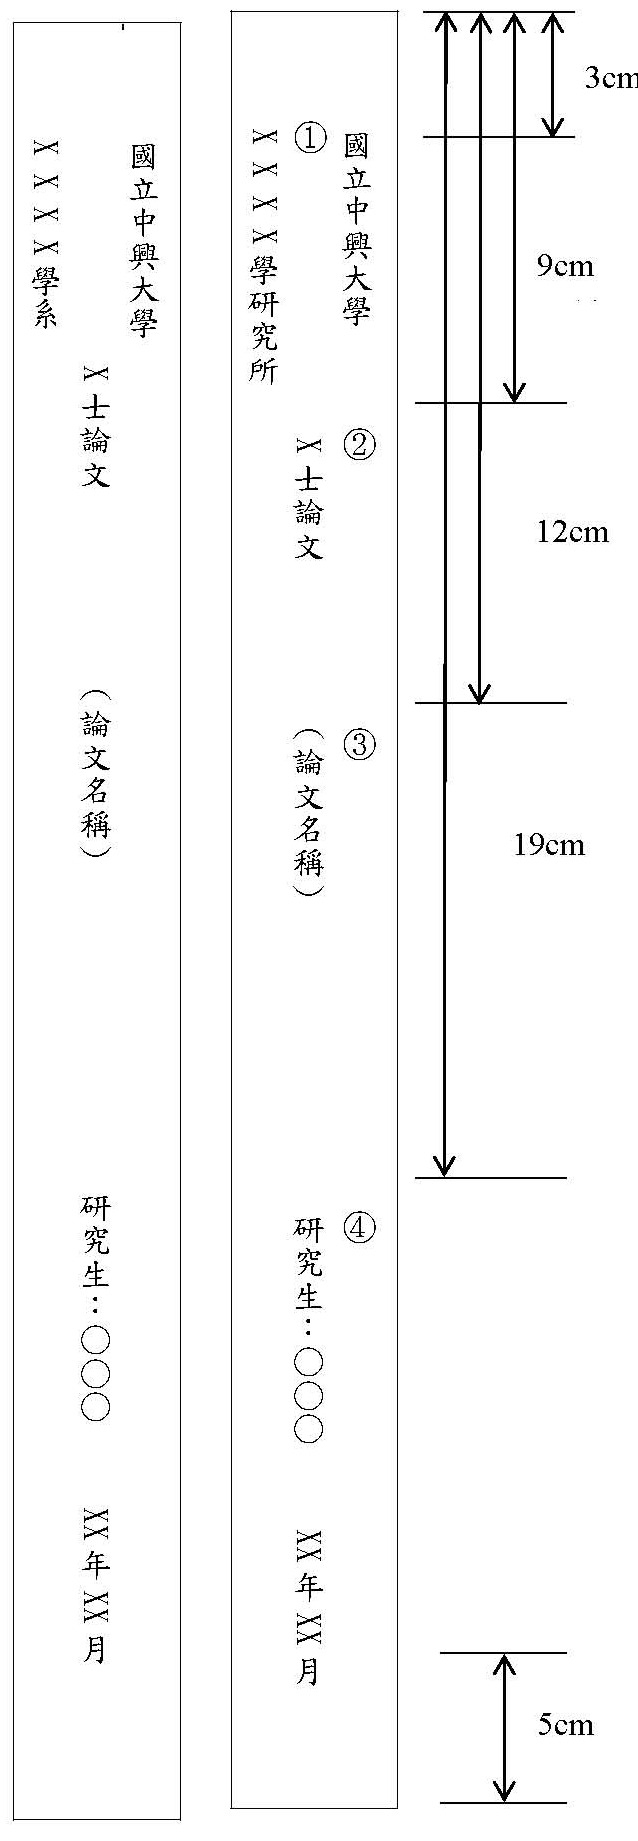
\includegraphics[bb=0 0 638 1841,width=0.45\textwidth]{ridge.jpg}
    \end{center}
\end{document}